Während die Fresnelsche und die Fraunhofersche Beugung die zwei \glqq{}klassischen\grqq{} Zugänge zur Theorie der Beugung bilden, ist die Fourieroptik ein weiterer Ansatz zu diesem Gebiet, welcher sich die mathematischen Werkzeuge der Fourieranalyse zunutze macht. Im Versuch 233 (bzw. 333) werden wir die Beugung von Licht am Einzel- und Doppelspalt vor dem Hintergrund der Fourieroptik betrachten.

\subsection{Physikalische Grundlagen}

\subsubsection*{Die Fraunhofersche Beugung}

Die Fresnelsche Beugung geht von endlichen Abständen zwischen Lichtquelle, Beugungsobjekt und Beobachtungsebene aus. Es treffen hierbei also Lichtstrahlen in verschiedensten Winkeln auf das Beugungsobjekt, entsprechend welcher sie gebeugt werden. Da die mathematische Beschreibung dieses Prinzips augenscheinlich sehr kompliziert ist, beschränken wir uns in diesem ersten Teil auf die Fraunhofersche Beugung.

Wie in \abbref{fig:fraunhofer_beugung} dargestellt, geht die Fraunhofersche Betrachtung der Beugung von unendlich großen Abständen zwischen Lichtquelle, Beugungsobjekt und Beobachtungsebene aus. In dieser Annäherung (\textit{bzw. Distanzierung lol}) treffen die Lichtstrahlen von der Quelle daher parallel und senkrecht auf das Beugungsobjekt. Da die gebrochenen Lichtbündel daher ebenfalls parallel sind, würden diese erst im Unendlichen interferieren (\ref{fig:fraunhofer_beugung}, links). Durch die Positionierung einer Sammellinse zwischen Beugungsobjekt und Beobachtungsebene (\ref{fig:fraunhofer_beugung}, rechts) lassen sich die Interferenzmuster bereits in der Entfernung der Brennweite der verwendeten Linse beobachten.

\begin{figure}[H]
  \centering
  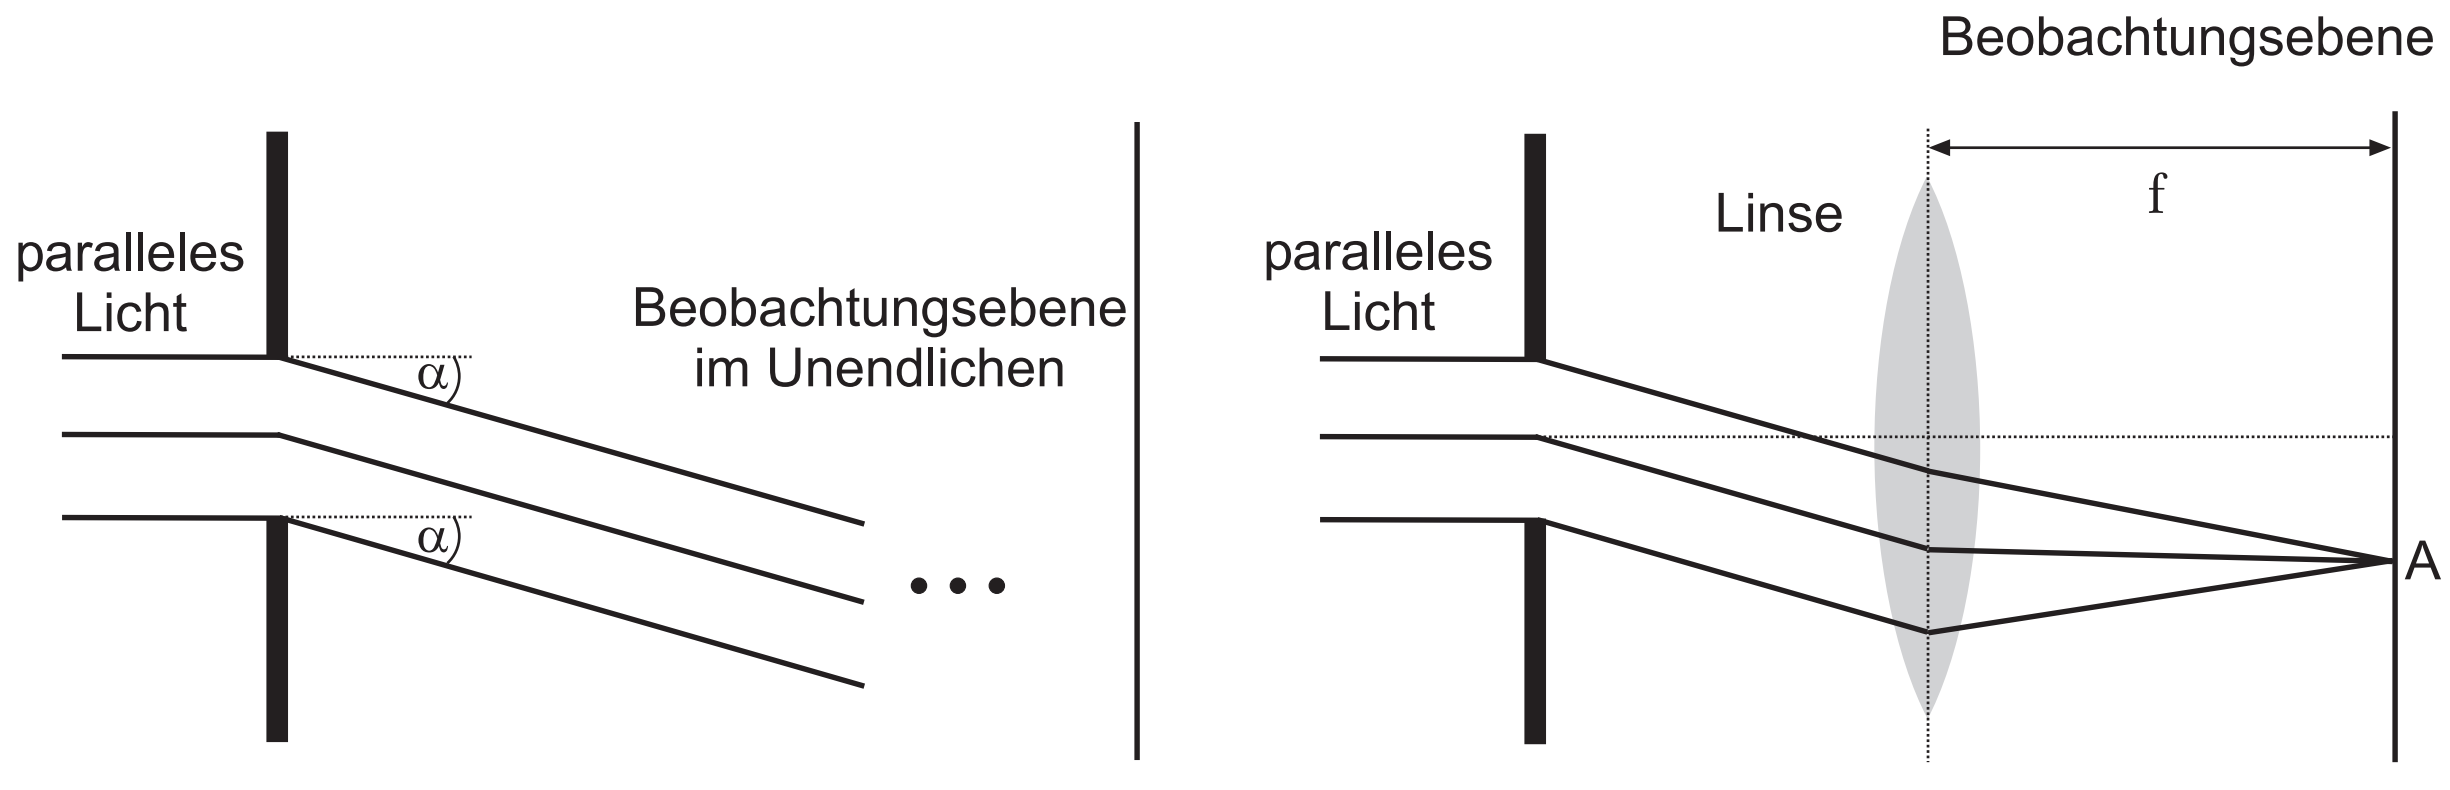
\includegraphics[width=.9\textwidth]{files/fraunhofer_beugung.png}
  \caption{Fraunhofersche Beugung mit Beobachtungsebene im Unendlichen (links) und in endlichem Abstand durch Verwendung einer Linse (rechts).}
  \label{fig:fraunhofer_beugung}
\end{figure}

Wir gehen nun von einem Spalt der Breite $d$ in y-Richtung, und einer Länge deutlich größer als $d$ aus. Alle Punkte des Spalts werden mit gleicher Amplitude $E_0$ und Phase $\varphi = \omega t$ von einem parallelen monochromatischen Lichtstrahl der Wellenlänge $\lambda$ erregt. Es gilt also
\begin{align}
  E(y) = E_0 \e{i\omega t}.
\end{align}

Das Huygens-Fermat'sche Prinzip besagt nun, dass von jedem dieser Punkte eine Elementarwelle ausgeht. Das Interferenzmuster dieser Wellen können wir bestimmen, indem wir die Überlagerung aller in einen bestimmten Winkel $\alpha$ ausgehenden Wellen betrachten. Mathematisch entspricht dies dem Integral
\begin{align}
    E_{\infty}(\alpha) = \int_{-\flatfrac{d}{2}}^{+\flatfrac{d}{2}} E_0 \e{i(\omega t - kl)} \dd y
\end{align}
mit dem Betrag des Wellenvektors $k = \frac{2\pi}{\lambda}$. 

\begin{figure}[H]
  \centering
  \begin{minipage}{0.65\textwidth}
    Der Gangunterschied zwischen einem Lichtbündel aus dem Mittelpunkt ($y = 0$) des Spalts und einem Lichtbündel abseits von diesem entspricht gerade $y \sin(\alpha)$. Somit gilt für die Weglänge des äußeren Bündels
    \begin{align}
      l = R + \sin(\alpha)
    \end{align}
    mit $R$ als Weglänge des Bündels aus dem Mittelpunkt. 
  \end{minipage}\hfill
  \begin{minipage}{0.3\textwidth}
      \centering
      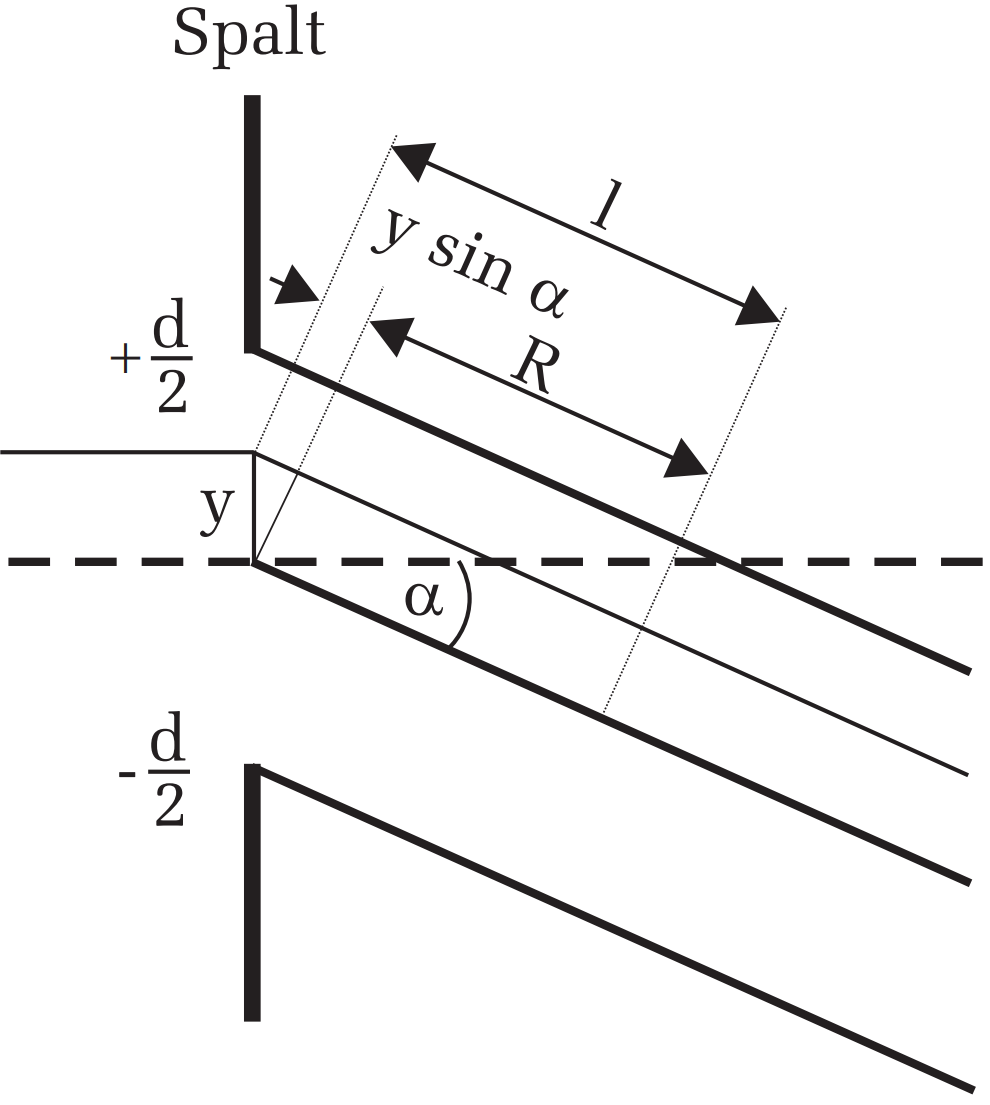
\includegraphics[width=0.9\textwidth]{files/gangunterschied_fraunhofer_einzelspalt.png}
      \caption{Gangunterschied der ausgehenden Lichtbündel am Einzelspalt.}
      \label{fig:gangunterschied_fraunhofer_einzelspalt}
  \end{minipage}
\end{figure}


Setzen wir diese Definition in das Integral ein, führen dieses aus und benutzen die Eulersche Formel für die e-Funktion, so ergibt sich
\begin{align}
  E_{\infty}(\alpha) = E_{0}\e{i(\omega t- kR)} \frac{\sin(\frac{\pi d \sin(\alpha)}{\lambda})}{\frac{\pi \sin(\alpha)}{\lambda}}.
\end{align}
\begin{figure}[H]
  \centering
  \begin{minipage}{0.55\textwidth}
    Wir identifizieren $x = \frac{d}{\lambda} \pi \sin(\alpha)$ und erhalten so
    \begin{align}
      E_{\infty}(x) = E_{0}\e{i(\omega t- kR)} \frac{\sin(x)}{x} d.
    \end{align}
    
    Durch das Quadrieren dieser Formel können wir die Intensität
    \begin{align}
      I_{\infty}(x) \propto \frac{\sin^2(x)}{x^2} d^2 \propto I_0 \frac{\sin^2(x)}{x}
    \end{align}
    mit $I_0 \propto d^2$ bestimmen. Diese ist dargestellt in \abbref{fig:intensitätsverteilung_fraunhofer_einzelspalt}.
  \end{minipage}\hfill
  \begin{minipage}{0.4\textwidth}
      \centering
      \includegraphics[width=0.9\textwidth]{files/intensitätsverteilung_fraunhofer_einzelspalt.png}
      \caption{Intensitätsverteilung der Beugungsstruktur des Einzelspalts.}
      \label{fig:intensitätsverteilung_fraunhofer_einzelspalt}
  \end{minipage}
\end{figure}

\subsubsection*{Fourierreihen und Fourierintegrale}

Eine Funktion $f: \R \to \R$ heißt periodisch, wenn ein $L \in \R$ existiert mit $f(x + L) = f(x)$ für alle $x \in \R$. Eine $L$-periodische und integrierbare Funktion lässt sich mit den trigonometrischen Funktionen
\begin{align}
  \cos(\frac{2\pi n}{L} x),\quad \sin(\frac{2\pi n}{L} x)\qquad n \in \N
\end{align}
als Basisvektoren entwickeln. Das heißt, es existieren $a_n, b_n \Forall n \in \N$ mit
\begin{align}
  f(x) = \frac{a_0}{2} + \sum_{n = 1}^{\infty} a_n \cos(\frac{2\pi n}{L} x) + b_n \sin(\frac{2\pi n}{L}) x.
\end{align}
Die sogenannten Fourierkoeffizienten $a_n$ und $b_n$ sind definiert durch 
\begin{align}
  a_n = \frac{2}{L} \int_{-\flatfrac{L}{2}}^{\flatfrac{L}{2}} f(x) \cos(\frac{2\pi n}{L} x) \dd x,
  \intertext{bzw.}
  b_n = \frac{2}{L} \int_{-\flatfrac{L}{2}}^{\flatfrac{L}{2}} f(x) \sin(\frac{2\pi n}{L} x) \dd x.
\end{align}

\subsection{Versuchsdurchführung}